\documentclass[12pt]{article}

\usepackage[active]{srcltx}

\usepackage{amsmath,amsfonts,amssymb,amsthm}
\usepackage{easybmat}
\usepackage{graphicx}
%\usepackage[hypertex]{hyperref}
%\usepackage[pdftex]{hyperref}
\usepackage{fancyhdr}
\usepackage{subfigure}

\usepackage{makeidx}
\makeindex

\theoremstyle{plain}
\newtheorem{theorem}{Theorem}[section]
\newtheorem{property}[theorem]{Property}
\newtheorem{condition}[theorem]{Condition}
\newtheorem{proposition}[theorem]{Proposition}
\newtheorem{axiom}[theorem]{Axiom}
\newtheorem{lemma}[theorem]{Lemma}
\newtheorem{corollary}[theorem]{Corollary}
%%
% % Make numbering specific to the Appendix
% \newtheorem{Atheorem}{Theorem}[chapter]
% \newtheorem{Aproperty}[Atheorem]{Property}
% \newtheorem{Acondition}[Atheorem]{Condition}
% \newtheorem{Aproposition}[Atheorem]{Proposition}
% \newtheorem{Aaxiom}[Atheorem]{Axiom}
% \newtheorem{Alemma}[Atheorem]{Lemma}
% \newtheorem{Acorollary}[theorem]{Corollary}

% Make definitions non italicized
%\theoremstyle{definition}
\newtheorem{definition}[theorem]{Definition}
% Make numbering specific to the Appendix
%\newtheorem{Adefinition}[Atheorem]{Definition}
\newenvironment{defi}{\vskip0.2cm\addtocounter{theorem}{1}\par\noindent\bf Definition~\arabic{section}.\arabic{subsection}.\arabic{theorem}\rm.}{\hfill{$\circ$}\par\vskip0.25cm}


%% Example environment and counter.
\newcounter{cmpt_exercise}
\newenvironment{exercise}{\addtocounter{cmpt_exercise}{1}\vskip0.2cm\par\noindent\begin{small}\bf Exercise~\arabic{cmpt_exercise}\,\,\rm --}{\hfill{$\circ$}\end{small}\par\vskip0.25cm}
\newenvironment{problem}{\addtocounter{cmpt_exercise}{1}\vskip0.2cm\par\noindent{\Large\bf Problem~\arabic{cmpt_exercise}\,\,\rm --}}{\par\vskip0.25cm}


\newenvironment{example}{\vskip0.2cm\par\noindent\begin{small}\bf Example\,\,\rm --}{\hfill{$\diamond$}\end{small}\par\vskip0.25cm}
\newenvironment{remark}{\vskip0.2cm\par\noindent\begin{small}\bf Remark\,\,\rm --}{\hfill{$\circ$}\end{small}\par\vskip0.25cm}
%\newenvironment{aparte}[1]{\vskip0.2cm\par\noindent\begin{quote}\begin{small}\bf Apart\'e : #1\,\,\rm --}{\hfill{$\circ$}\end{small}\end{quote}\par\vskip0.25cm}
\newenvironment{aparte}[1]{\vskip0.3cm\par\begin{center}\begin{tabular}{|p{0.9\textwidth}|}\hline{\bf Apart\'e : #1}}{\\ \hline\end{tabular}\end{center}\par\vskip0.25cm}

\renewcommand{\labelenumi}{\roman{enumi})}
\renewcommand{\labelenumii}{\alph{enumii})}
\newcommand{\espv}{\vspace{.5\baselineskip}}
\def\IR{\mathbb{R}}
\def\IC{\mathbb{C}}
\def\IN{\mathbb{N}}
\def\IQ{\mathbb{Q}}
\def\IZ{\mathbb{Z}}
\def\rank{\textrm{rank }}
\def\Sp{\textrm{Sp }}
\def\Span{\textrm{Span }}
\def\Tr{\textrm{Tr }}
\def\D{\mathcal{D}}
\def\I{\mathcal{I}}
\def\U{\mathcal{U}}
\def\R{\mathcal{R}}
\def\Q{\mathcal{Q}}
\def\O{\mathcal{O}}
\def\Mn{\mathcal{M}_n}
\def\NN#1{\|#1\|}
\def\N3#1{|\!|\!|#1|\!|\!|}
\def\diag{\textrm{diag}}
\def\tr{\textrm{tr}}
\def\ker{\textrm{Ker }}

\def\M{\mathcal{M}}

\setlength{\textwidth}{17cm} 
\addtolength{\oddsidemargin}{-1.5cm}
\setlength{\textheight}{22cm}
\addtolength{\topmargin}{-2cm} 
\setlength{\headheight}{25.3pt}

%% Fancyhdr related stuff
\pagestyle{fancy}
\lhead{J. Arino -- MATH 3820 -- Modelling}
\rhead{\thepage}

\usepackage[hang,small,bf]{caption2}
\setlength{\captionmargin}{20pt}

\makeatletter
\def\cleardoublepage{\clearpage\if@twoside \ifodd\c@page\else
\hbox{}
% \vspace*{\fill}
% \begin{center}
% This page intentionally contains only this sentence.
% \end{center}% Make numbering specific to the Appendix
\newtheorem{Atheorem}{Theorem}[chapter]
\newtheorem{Aproperty}[Atheorem]{Property}
\newtheorem{Acondition}[Atheorem]{Condition}
\newtheorem{Aproposition}[Atheorem]{Proposition}
\newtheorem{Aaxiom}[Atheorem]{Axiom}
\newtheorem{Alemma}[Atheorem]{Lemma}
\newtheorem{Acorollary}[theorem]{Corollary}

% \vspace{\fill}
\thispagestyle{empty}
\newpage
\if@twocolumn\hbox{}\newpage\fi\fi\fi}
\makeatother

%\author{Julien Arino}
%\address{University of Manitoba}
%\title{MATH 8430\\ Lecture Notes}
\title{The logistic map}
\author{Julien Arino}

%%%%%%%%%%%%%%%%
%%%%%%%%%%%%%%%%
%%%%%%%%%%%%%%%%
%%%%%%%%%%%%%%%%
%%%%%%%%%%%%%%%%
%%%%%%%%%%%%%%%%
\begin{document}

\maketitle

\begin{abstract}
This details the analysis of the logistic map as done in class, and adds additional considerations. Computations are carried out explicitly up to the existence of period 2 points.
\end{abstract}

We consider the logistic map
\begin{equation}\label{eq:logistic_map}
f_\mu(x)=\mu x(1-x),
\end{equation}
used to define the discrete time logistic equation
\begin{equation}
x_{t+1}=f_\mu(x_t), \label{eq:logistic}
\end{equation}
the latter being considered with initial condition $x_0\in[0,1]$. It is assumed throughout that $0<\mu<4$.

\section{Well-posedness}
We consider the case $0<\mu<4$, where we know for certain that the iterates of $f_\mu$ remain in the set $[0,1]$. Indeed, 
\begin{equation}\label{eq:dlogistic_map}
f_\mu'(x)=\mu-2\mu x=\mu(1-2x),
\end{equation}
so $f_\mu$ is increasing for $x<1/2$ and decreasing for $x>1/2$, with a maximum at $x=1/2$, equal to $\mu/4$. On the other hand, $f_\mu(0)=f_\mu(1)=0$, so the minima are at $x=0$ and $x=1$. Therefore, if $\mu<4$ then $f_\mu([0,1])\subset[0,1]$.

\section{Fixed points of $f_\mu$}
Fixed points of \eqref{eq:logistic_map} are found by solving the fixed point equation
\[
f_\mu(x)=x,
\]
that is,
\[
\mu x(1-x)=x.
\]
It is clear that there are two points that satisfy this equation, namely $x=0$ and $x=(\mu-1)/\mu$. We denote from now on $p=(\mu-1)/\mu$.

Note that $x=0$ always exists. On the other hand, $p$ has the following properties:
\begin{itemize}
\item $\lim_{\mu\to 0^+}p=-\infty$.
\item $\dfrac{\partial}{\partial \mu}p=\dfrac{1}{\mu^2}>0$, so $p$ is an increasing function of $\mu$.
\item $p=0$ if and only if $\mu=1$ (unique since $p$ is increasing).
\item $\lim_{\mu\to\infty}p=1$.
\end{itemize}
Remember that we are modelling a population, so we want $p>0$ (or at least, nonnegative). If $p>0$, we say that $p$ is \emph{biologically relevant}. For this, we need $\mu>1$. In the case that $\mu<1$, then $p$ does exist, but we do not consider it, as it is not biologically relevant, and by abuse of language, say that $p$ does not exist.

\vskip0.5cm
\noindent{\bf Conclusion 1.} We conclude, at this point, that the situation is as follows. The fixed point $x=0$ always exists, and
\begin{itemize}
\item if $\mu\in(0,1)$, then $p$ does not exist,
\item if $\mu>1$, then $p$ exists.
\end{itemize}


\section{Stability of the fixed points}
To determine the stability of $f_\mu$ at a fixed point $x^*$, we need to compare $|f'_\mu(x^*)|$ with the value 1. From \eqref{eq:dlogistic_map},
\[
|f_\mu'(0)|=|\mu|=\mu,
\]
and
\begin{align*}
|f_\mu'(p)| &= \left|\mu\left(1-2\frac{\mu-1}{\mu}\right)\right| \\
&= |1-2\mu|.
\end{align*}
As a consequence, $x=0$ is attracting if $\mu<1$ and repelling otherwise, and $p=(\mu-1)/\mu$ is attracting if $1-2\mu<1$, that is, $\mu<3$, and repelling otherwise.

\vskip0.5cm
\noindent{\bf Conclusion 2.} Building upon {\bf Conclusion 1}, we therefore deduce that
\begin{itemize}
\item if $\mu\in(0,1)$, then $x=0$ is attracting, and the fixed point $x=p$ does not exist,
\item if $\mu\in(1,3)$, then $x=0$ is repelling, and the fixed point $x=p$ exists and is attracting,
\item if $\mu>3$, then $x=0$ is repelling, and the fixed point $x=p$ exists and is repelling.
\end{itemize}


\begin{remark}
A fixed point that is such that $|f'(p)|\neq 1$, or a periodic point such that $|(f^k)'(p)|\neq 1$, is called \emph{hyperbolic}. In the case that $|f'(p)|=1$, or, for a periodic point, $|(f^k)'(p)|=1$, then $p$ is called \emph{non hyperbolic}. The non hyperbolic case is harder to treat. Here, the case $\mu=1$ is a \emph{non hyperbolic} case. However, the probability that $\mu=1$ is zero (the set $\mu=\{1\}$ has measure zero in the parameter space $\IR_+$), explaining why, most of the time, the case $\mu=1$ is omitted.
\end{remark}



\section{Stable sets of the fixed points}
{\bf Conclusion 2} establishes that $x=0$ and $x=p$ are attracting when, respectively, $\mu\in(0,1)$ and $\mu\in(1,3)$. This is not sufficient to characterize the behavior of all solutions. Remember that attractiveness of a fixed point $x^*$ implies that there is a neighborhood of $x^*$ that belongs to $W^s(x^*)$, i.e., there exists 
a neighborhood $\mathcal{N}\ni x^*$ such that $\forall x\in\mathcal{N}$, $x$ is forward asymptotic to $x^*$.

If we want to make sure that we have the ``complete picture'', we need to show that $W^s(x^*)=[0,1]$, i.e., that all solutions go to $x^*$. There are several ways to tackle this problem, only one is shown here.

\subsection{Case of the fixed point $x=0$ (i.e., case $0<\mu<1$)}
Since $\mu<1$, it follows that $f_\mu(x)=\mu x(1-x)<x(1-x)$ Also, $x\in[0,1]$ implies that $1-x\in[0,1]$, and therefore $f_\mu(x)<x(1-x)\leq x$. Therefore, for any $x_0\in[0,1]$,
\begin{align*}
x_1 &= f_\mu(x_0) \\
&< x_0 \\
x_2 &= f_\mu(x_1) \\
& < x_1.
\end{align*}
Therefore we have a strictly decreasing sequence. Since $[0,1]$ is invariant, the sequence is bounded below by $0$. Therefore $\lim_{k\to\infty}f^k(x_0)=0$, and $W^s(0)=[0,1]$ when $0<\mu<1$. Therefore we can strengthen {\bf Conclusion 2}.

\noindent{\bf Conclusion 3$'$.} If $0<\mu<1$, then for all $x_0\in[0,1]$, $\lim_{k\to\infty}f^k(x_0)=0$, or, equivalently, $\lim_{t\to\infty}x_t=0$.

\begin{remark}
In the considerations above, we could have used Theorem~\ref{th:gas_1} directly, once it was established that $f_\mu(x)<x$.
\end{remark}
 

\subsection{Case of the fixed point $x=p$ (i.e., case $1<\mu<3$)}
We know that $f_\mu$ is increasing from a minimum of 0 at $x=0$ to a maximum $\mu/4$ at $x=1/2$, and then decreasing from there to a minimum of 0 at $x=1$. Therefore, we must distinguish two cases: $\mu<2$ and $\mu>2$.


\subsubsection{Case $1<\mu<2$}
In the case $\mu<2$, the intersection of $f_\mu(x)$ with the first bisectrix $x$ occurs before the maximum $\mu/4$ is reached (see Figure~\ref{fig:logistic_1dot5}).
\begin{figure}[htbp]
\begin{center}
\includegraphics[width=0.5\textwidth]{logistic_1dot5}
\end{center}
\caption{The function $f_{1.5}(x)$.}\label{fig:logistic_1dot5}
\end{figure}
Then we are in a position to use part {\bf a} in Theorem~\ref{th:gas_4}, giving the conclusion.

\subsubsection{Case $2<\mu<3$}
In the case $\mu>2$, the intersection of $f_\mu(x)$ with the first bisectrix $x$ occurs after the maximum $\mu/4$ is reached (see Figure~\ref{fig:logistic_2dot5}).
\begin{figure}[htbp]
\begin{center}
\includegraphics[width=0.5\textwidth]{logistic_2dot5}
\end{center}
\caption{The function $f_{2.5}(x)$.}\label{fig:logistic_2dot5}
\end{figure}
We use Theorem~\ref{th:gas_2} in Appendix~\ref{sec:global_stability}. In order to be able to apply this theorem, we must first prove that there are no 2-cycles. For this purpose, we could try to use Theorem~\ref{th:no_cycles}, but it fails to provide the conclusion here. Here, we can use the result from Section~\ref{sec:2cycles}, where it is shown by explicit calculation that there are no 2-cycles for $\mu<3$.

It is clear that $f$ satisfies the hypotheses of Theorem~\ref{th:gas_2}. Indeed, $f$ is decreasing for $x>1/2$.

\begin{remark}
We could also have used part {\bf b} in Theorem~\ref{th:gas_4}, but this required to show that $f^2(x)>x$ for $x\in(1/2,p)$.
\end{remark}


\subsubsection{Case $\mu=2$}
The result used to treat the case $\mu<2$ can, in the present case, be extended to include the case where $\mu=2$.


% Here, the first idea would be to show the following:
% \begin{itemize}
% \item if $x_0\in(0,p)$, then $\{x_k\}$ is an increasing sequence,
% \item if $x_0\in(p,1)$, then $\{x_k\}$ is a decreasing sequence.
% \end{itemize}
% Note, however, that this is not sufficient: clearly, nothing forbids the sequence from ``jumping'' from one side of $p$ to the other. This is easy to see using cobwebbing: choosing $x_0$ such that $f_\mu(x_0)>p$ is not difficult (if suffices to choose $x_0$ such that $f_\mu(x_0)$ is above the line $y=p$). We thus want to show that the jumps take us closer and closer to $p$.
% 
% To do this, we consider the interval $I_0=(\varepsilon,1)$, with $\varepsilon>0$ small. We have $f_\mu'(0)=\mu>1$, and by continuity of $f_\mu'$, it is therefore possible to choose $\varepsilon$ small enough that $f_\mu'(\varepsilon)=\mu(1-2\varepsilon)>1$.


\section{Points of period 2}
\label{sec:2cycles}
We now study the existence of periodic points with least period 2, that is, fixed points of the map $f_\mu^2(x)$. We have
\begin{align}
f_\mu^2(x) &= f_\mu(f_\mu(x)) \nonumber\\
&= \mu f_\mu(x)(1-f_\mu(x)) \nonumber\\
&= \mu^2 x(1-x)(1-\mu x(1-x)). \label{eq:f_mu_2_a}
\end{align}
Remark that 0 and $p$ are points of period 2. Indeed, a fixed point $x^*$ of $f$ satisfies $f(x^*)=x^*$, and as a consequence, $f^2(x^*)=f(f(x^*))=f(x^*)=x^*$. This is extremely helpful in localizing the other periodic points, if there are any. Indeed, writing the fixed point equation as
\[
f_\mu^2(x)-x=0,
\]
and defining $Q(x):=f_\mu^2(x)-x$, we see that, since $0$ and $p$ are fixed points of $f_\mu^2$, they are roots of $Q(x)$. Therefore, $Q$ can be factorized as
\[
Q(x)=x(x-p)(-\mu^3x^2+Bx+C),
\]
since it is clear from \eqref{eq:f_mu_2_a} that $f_\mu^2$ is a polynomial of degree 4 with leading coefficient equal to $-\mu^3$. Substituting the value $(\mu-1)/\mu$ for $p$ in $Q$, developing $Q$ and \eqref{eq:f_mu_2_a} and equating coefficients of like powers gives
\begin{equation}\label{eq:Q}
Q(x)=x\left(x-\frac{\mu-1}{\mu}\right)\left(-\mu^3 x^2+\mu^2(\mu+1)x-\mu(\mu+1)\right).
\end{equation}
The roots of \eqref{eq:Q} are the fixed points of $f_\mu^2$. Since $x=0$ and $x=p$ are already known, we can concentrate on the roots of the polynomial
\[
R(x):=-\mu^3 x^2+\mu^2(\mu+1)x-\mu(\mu+1).
\]
The discriminant is $\Delta=\mu^4(\mu+1)^2-4\mu^4(\mu+1)=\mu^4(\mu+1)(\mu+1-4)=\mu^4(\mu+1)(\mu-3)$. Therefore, $R$ has distinct real roots if $\mu>3$, and a double real root if $\mu=3$. In the latter case, the root is
\[
\frac{-\mu^2(\mu+1)}{-2\mu^3}=\frac{\mu+1}{2\mu}=\frac 23,
\]
which is the value of $p$ when evaluated at $\mu=3$: the fixed point $p$ and the fixed point deduced from $R$ coincide at $\mu=3$.

\vskip1cm
So we now consider the case $\mu>3$. In this case, $R$ has two distinct real roots (that is, $f_\mu^2$ has two distinct real fixed points). More than their actual value, what is of interest is 
\begin{enumerate}
\item are these roots positive,
\item are these roots smaller than 1.
\end{enumerate}
If one or both of them is not in $(0,1)$, it will indeed have to be considered as non biologically relevant and ignored.

First, remark that for $\mu>3$ but very close to 3, it follows from the continuity of $R$ that the roots are in $(0,1)$.
To show that this is still the case as we move away from 3, we use Descartes' rule of signs (Theorem~\ref{th:descartes}, Appendix~\ref{sec:descartes}). For this, remark that $R$ has signed coefficients $-+-$, giving two sign changes and the possibility of 0 or 2 positive real roots. On the other hand, $R(-x)$ has signed coefficients $---$, hence there are no negative real roots. As we are in the case where the roots are real, it follows that both roots are positive.

To show that the roots are also smaller than 1, consider the change of variables $z=x-1$. The polynomial $R$ is transformed into 
\begin{align*}
R_2(z) &= -\mu^3 (z+1)^2+\mu^2(\mu+1)(z+1)-\mu(\mu+1) \\
&= -\mu^3z^2+\mu^2(1-\mu)z-\mu.
\end{align*}
For $\mu>1$, all the coefficients of this polynomial are negative, implying that $R_2$ has no root $z>0$, implying in turn that $R$ has no root $x>1$.


% \section{Attractiveness of the periodic orbits}
% \[
% \left(f_\mu^2\right)'(x)=-\mu^2(2x-1)(2\mu x^2-2\mu x+1)
% \]

\section{The cascade of bifurcation to chaos}
\label{sec:chaos}
Sharkovskii's ordering of integers is as follows:
\begin{gather*}
3\triangleright 5\triangleright 7 \triangleright 9 \triangleright 11\triangleright \cdots \triangleright 2\cdot 3\triangleright  2\cdot 5\triangleright \cdots \triangleright 2\cdot 9\triangleright\cdots\triangleright 2^2\cdot 3\triangleright 2^2\cdot 5\triangleright \cdots \\
\triangleright 2^n\cdot 3\triangleright 2^n\cdot 5\triangleright \cdots\triangleright 2^{n+1}\cdot 3\triangleright 2^{n+1}\cdot 5\triangleright \cdots
\triangleright 2^{n+1}\triangleright 2^n\triangleright \cdots 2^2 \triangleright 2\triangleright 1.
\end{gather*}
This gives an ordering between all positive integers. The following result helps characterizing the behavior of the cascade.
\begin{theorem}[Sharkovskii]\label{th:sharkovskii}
Let $f:I\subset\IR\to\IR$ be a continuous function. Assume that $f$ has a point of least period $n$ and $n\triangleright k$. Then $f$ has a point of least period $k$.
\end{theorem}


\begin{figure}[htbp]
\begin{center}
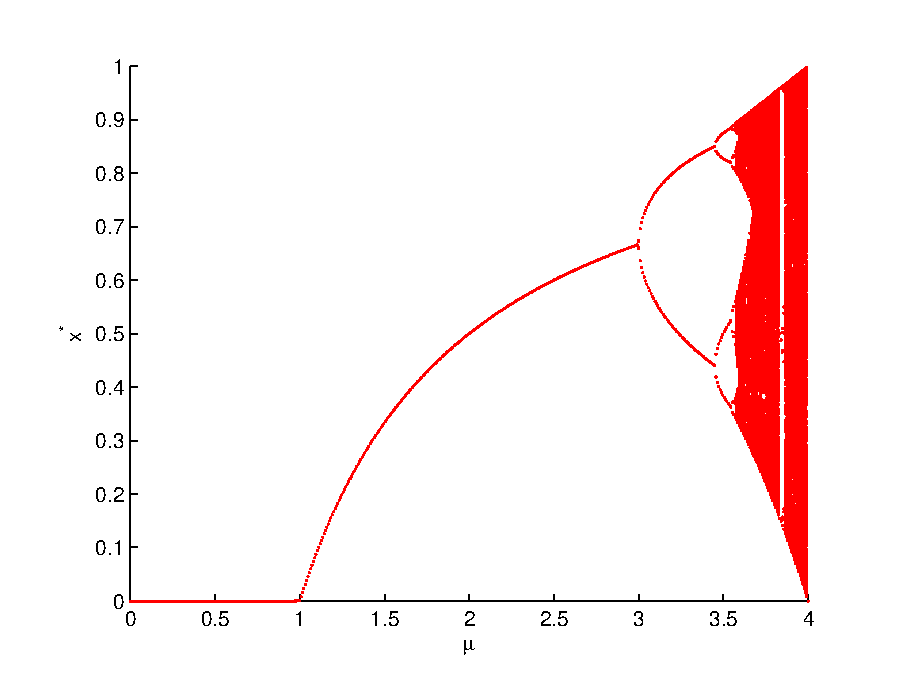
\includegraphics[width=0.5\textwidth]{analysis_logistic_cascade_full}
\end{center}
\caption{The cascade of bifurcation to chaos for the logistic map.}
\end{figure}



%%%%%%%%%%
%%%%%%%%%%
\bibliographystyle{plain}
\bibliography{bib_logistic}

\appendix
\section{Descartes' rule of signs}
\label{sec:descartes}
\begin{theorem}[Descartes' rule of signs]\label{th:descartes}
Let $p(x) = \sum_{i=0}^m a_ix^i $ be a polynomial with real coefficients such that $a_m \neq 0$.
Define $v$ to be the number of {\it variations in sign} of the sequence of coefficients $a_m, \ldots, a_0$. By 'variations in sign' we mean the number of values of $n$ such that the sign of $a_n$ differs from the sign of $a_{n - 1}$, as $n$ ranges from $m$ down to 1.
Then 
\begin{itemize}
\item the number of positive real roots of $p(x)$ is $v-2N$ for some integer $N$ satisfying $0 \leq N \leq \dfrac{v}{2}$,
\item the number of negative roots of $p(x)$ may be obtained by the same method by applying the rule of signs to $p(-x)$.
\end{itemize}
\end{theorem}


\begin{example}
Let $p(x) = x^3+3x^2-x-3$. The coefficients have sign $++--$, so there is one sign change.
Thus $v = 1$. Since $0 \leq N \leq 1/2$, we must have $N=0$. Thus $v-2N=1$ and there is exactly one positive real root of $p(x)$.

To find the negative roots, we examine $p(-x) = -x^3+3x^2+x-3$. The coefficients have sign $-++-$, so there are two sign changes. Thus $v=2$ and $0 \leq N \leq 2/2= 1$.
Thus, there are two possible solutions, $N=0$ and $N=1$, and two possible values of $v-2N$. Therefore, there are either two or no negative real roots.
Furthermore, note that $p(-1)=(-1)^3+3 \cdot (-1)^2-(-1)-3=0$, hence there is at least one negative root. Therefore there must be exactly two.
\end{example}

\section{Global stability}
\label{sec:global_stability}
The results presented here come from \cite{Allen2007}. We use the words \emph{equilbrium} and \emph{fixed point} interchangeably. Throughout this Appendix, we consider the discrete time scalar equation
\begin{equation}\label{sys}
x_{t+1}=f(x_t)
\end{equation}
induced by the mapping $f$.

\begin{definition}[Globally attractive fixed point]
Suppose that $\bar x$ is a fixed point of $f$,
where $f: [0,a)\rightarrow [0,a),$ $0<a\leq \infty$. Then $\bar x$ is said to be \emph{globally attractive} if for all initial conditions $x_0\in (0,a)$, $$\lim_{t\rightarrow \infty}x_t=\bar x.$$
\end{definition}

\begin{definition}[Globally asymptotically stable fixed point]
The fixed point is said to be \emph{globally asymptotically stable} if $\bar x$ is globally attractive and if $\bar x$ is locally stable.
\end{definition}
Globally attractive equilibria are locally attractive, therefore globally asymptotically stable equilibria are locally asymptotically stable.


\begin{theorem}\label{th:gas_1}
If the function $f$ satisfies
\begin{enumerate}
\item $f$ is continuous on $[0,a),$ $0<a\leq \infty$,
\item $f: [0,a)\rightarrow [0,a),$ $0<a\leq \infty$,
\item $0<f(x)<x$ for all $x\in [0,a)$,
\end{enumerate}
then the origin is globally asymptotically stable for \eqref{sys}.
\end{theorem}

\begin{theorem}\label{th:gas_2}
The difference equation \eqref{sys}, with $f$ satisfying 
\begin{enumerate}
\item $f$ is continuous on $[0,a),$ $0<a\leq \infty$,
\item $f: [0,a)\rightarrow [0,a),$ $0<a\leq \infty$,
\item $f(0)=0$, $f(\bar x)=\bar x$ ,
\item $f(x)>x$ for $0<x<\bar x$,
\item $f(x)<x$ for $\bar x<x<a$,
\item if $f$ has a maximum at $x_M$ in $(0,\bar x)$, then $f$ is decreasing for $x>x_M$,
\end{enumerate}
has a globally asymptotically stable equilibrium at $\bar x$ if and only if has no 2-cycles.
\end{theorem}

To prove that there are no 2-cycles, the next result is helpful.
\begin{theorem}\label{th:no_cycles}
Let $f'$ be continuous on an interval $I$ and $f: I\rightarrow I$. If $1+f'(x)\not =0$ for all $x\in I$ then \eqref{sys} has no $2-cycles$ in $I$.
\end{theorem}

\begin{theorem}\label{th:gas_3}
If $f$ satisfies
\begin{enumerate}
\item $f$ is continuous on $[0,a),$ $0<a\leq \infty$,
\item $f: [0,a)\rightarrow [0,a),$ $0<a\leq \infty$,
\item $\bar x \in (0,a)$ such that $x<f(x)<\bar x$ for $0<x<\bar x$
and $\bar x<f(x)< x$ for $x>\bar x$
\end{enumerate}
then the difference equation \eqref{sys} has a globally asymptotically stable equilibrium at $\bar x$.
\end{theorem}

\begin{theorem}\label{th:gas_4}
Consider the difference equation \eqref{sys}.
\begin{description}
\item[a.]Suppose that $f$ satisfies
\begin{enumerate}
\item $f$ is continuous on $[0,a),$ $0<a\leq \infty$,
\item $f: [0,a)\rightarrow [0,a),$ $0<a\leq \infty$,
\item $f(0)=0$, $f(\bar x)=\bar x$ 
\item $f(x)>x$ for $0<x<\bar x$
\item $f(x)<x$ for $\bar x<x<a$
\end{enumerate}
but has no maximum in $(0,\bar x)$. Then $\bar x$ is globally asymptotically stable.
\item[b.]Suppose that $f$ satisfies
\begin{enumerate}
\item $f$ is continuous on $[0,a),$ $0<a\leq \infty$,
\item $f: [0,a)\rightarrow [0,a),$ $0<a\leq \infty$,
\item $f(0)=0$, $f(\bar x)=\bar x$ 
\item $f(x)>x$ for $0<x<\bar x$
\item $f(x)<x$ for $\bar x<x<a$
\item if $f$ has a maximum at $x_M$ in $(0,\bar x)$, then $f$ is decreasing for $x>x_M$
\end{enumerate}
has a maximun $x_M$ in $(0,\bar x)$. Then $\bar x$ is globally asymptotically stable if and only if $f^2(x)>x$ for all $x\in [x_M,\bar x)$
\end{description}
\end{theorem}


\end{document}
